\begin{figure}[t]
\centering
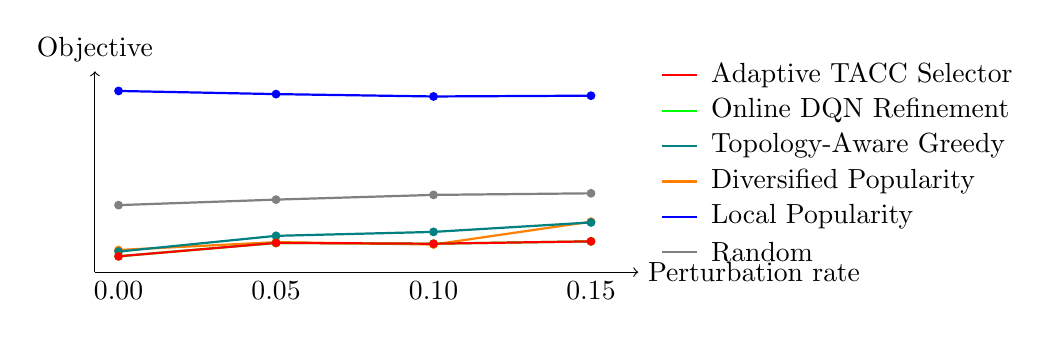
\begin{tikzpicture}[x=1cm,y=1cm]
\draw[->] (0.7,0.55) -- (7.6,0.55) node[right] {Perturbation rate};
\draw[->] (0.7,0.55) -- (0.7,3.1) node[above] {Objective};
\node[below] at (1.00,0.55) {0.00};
\node[below] at (3.00,0.55) {0.05};
\node[below] at (5.00,0.55) {0.10};
\node[below] at (7.00,0.55) {0.15};
\draw[gray, thick] (1.00,1.40) -- (3.00,1.47) -- (5.00,1.53) -- (7.00,1.55);
\fill[gray] (1.00,1.40) circle (1.6pt);
\fill[gray] (3.00,1.47) circle (1.6pt);
\fill[gray] (5.00,1.53) circle (1.6pt);
\fill[gray] (7.00,1.55) circle (1.6pt);
\draw[gray, thick] (7.9,0.80) -- (8.35,0.80);
\node[right] at (8.4,0.80) {Random};
\draw[blue, thick] (1.00,2.85) -- (3.00,2.81) -- (5.00,2.78) -- (7.00,2.79);
\fill[blue] (1.00,2.85) circle (1.6pt);
\fill[blue] (3.00,2.81) circle (1.6pt);
\fill[blue] (5.00,2.78) circle (1.6pt);
\fill[blue] (7.00,2.79) circle (1.6pt);
\draw[blue, thick] (7.9,1.25) -- (8.35,1.25);
\node[right] at (8.4,1.25) {Local Popularity};
\draw[orange, thick] (1.00,0.83) -- (3.00,0.93) -- (5.00,0.90) -- (7.00,1.19);
\fill[orange] (1.00,0.83) circle (1.6pt);
\fill[orange] (3.00,0.93) circle (1.6pt);
\fill[orange] (5.00,0.90) circle (1.6pt);
\fill[orange] (7.00,1.19) circle (1.6pt);
\draw[orange, thick] (7.9,1.70) -- (8.35,1.70);
\node[right] at (8.4,1.70) {Diversified Popularity};
\draw[teal, thick] (1.00,0.81) -- (3.00,1.01) -- (5.00,1.06) -- (7.00,1.18);
\fill[teal] (1.00,0.81) circle (1.6pt);
\fill[teal] (3.00,1.01) circle (1.6pt);
\fill[teal] (5.00,1.06) circle (1.6pt);
\fill[teal] (7.00,1.18) circle (1.6pt);
\draw[teal, thick] (7.9,2.15) -- (8.35,2.15);
\node[right] at (8.4,2.15) {Topology-Aware Greedy};
\draw[green, thick] (1.00,0.75) -- (3.00,0.92) -- (5.00,0.91) -- (7.00,0.94);
\fill[green] (1.00,0.75) circle (1.6pt);
\fill[green] (3.00,0.92) circle (1.6pt);
\fill[green] (5.00,0.91) circle (1.6pt);
\fill[green] (7.00,0.94) circle (1.6pt);
\draw[green, thick] (7.9,2.60) -- (8.35,2.60);
\node[right] at (8.4,2.60) {Online DQN Refinement};
\draw[red, thick] (1.00,0.75) -- (3.00,0.92) -- (5.00,0.91) -- (7.00,0.94);
\fill[red] (1.00,0.75) circle (1.6pt);
\fill[red] (3.00,0.92) circle (1.6pt);
\fill[red] (5.00,0.91) circle (1.6pt);
\fill[red] (7.00,0.94) circle (1.6pt);
\draw[red, thick] (7.9,3.05) -- (8.35,3.05);
\node[right] at (8.4,3.05) {Adaptive TACC Selector};
\end{tikzpicture}
\caption{Objective value under topology perturbation. Adaptive TACC selects among diversity-aware placement, topology-aware greedy, and online DQN refinement using held-out perturbation samples, relocation cost, and validation variability.}
\label{fig:objective_perturbation}
\end{figure}
